\section{Application Implementations}
\label{appendix:appl-impl}

Below we provide details about how we implement our applications, including the
libraries we use and how we integrate them into \sysname{}.

\para{Augmented Reality.} We target mobile augmented reality applications that
recognizes objects by offloading the heavy computation to resources elsewhere.
We implement image-related operations with OpenCV 3.1~\cite{opencvlibrary} and
recognize objects using YOLO~\cite{darknet13, redmon2016yolo9000}, a GPU-enabled
pre-trained neural network. Video encoding employs H.264 because of its
prevalence in existing systems. Our implementation uses
GStreamer~\cite{gstreamer} with \texttt{x264enc} plugin. To integrate with
\sysname{}, we first create a pipeline that exposes \texttt{appsrc} (to feed raw
image data) and \texttt{appsink} (to get encoded bytes). The GStreamer main loop
executes in a separate thread and \sysname{} communicates with it via Rust's
channel. The \texttt{x264enc} uses the \texttt{zerolatency} preset and four
threads. We use constant quality encoding and expose the quantization factor as
another knob (in addition to image resolution and frame rate).

Object recognition returns a list of bounding boxes with the type of the object,
and each box is a rectangle with normalized coordinates on the image. We compare
the detection against the reference result from raw data, and declare it success
if the intersection over union (IOU) is greater than
50\%~\cite{everingham2010pascal} and the object type matches. We use F1 score
(\%)~\cite{Rijsbergen:1979:IR:539927} as the accuracy function. In terms of
dataset, we've collected our own video clips: the training data is a 24-second
long video of an office environment; the test data is a 246-second long video of
a home environment.

\para{Pedestrian Detection.} This application analyzes streams of videos from
installed CCTV cameras and detects pedestrians inside. We use a similar setup
(OpenCV and GStreamer) as our augmented reality application except for the
analytical function. To detect pedestrians, we use histogram of oriented
gradients (HOG)~\cite{dalal2005histograms} with the default linear SVM
classifier. To ensure real-time processing of frames, we use the GPU-accelerated
implementation. Because we do not recognize individual pedestrians, a successful
detection in this case only requires matching the bounding box.  MOT16
dataset~\cite{milan2016mot16} is used for both training and testing.

\para{Distributed Top-K.} Many monitoring applications need to answer the
\textit{Top-K} question~\cite{babcock2003distributed}, such as the Top-K most
popular URLs, or the Top-K most access files. A distributed Top-K application
aggregates information from geo-distributed servers to computer a final Top-K
(\autoref{fig:topk}).

\begin{figure}
  \centering
  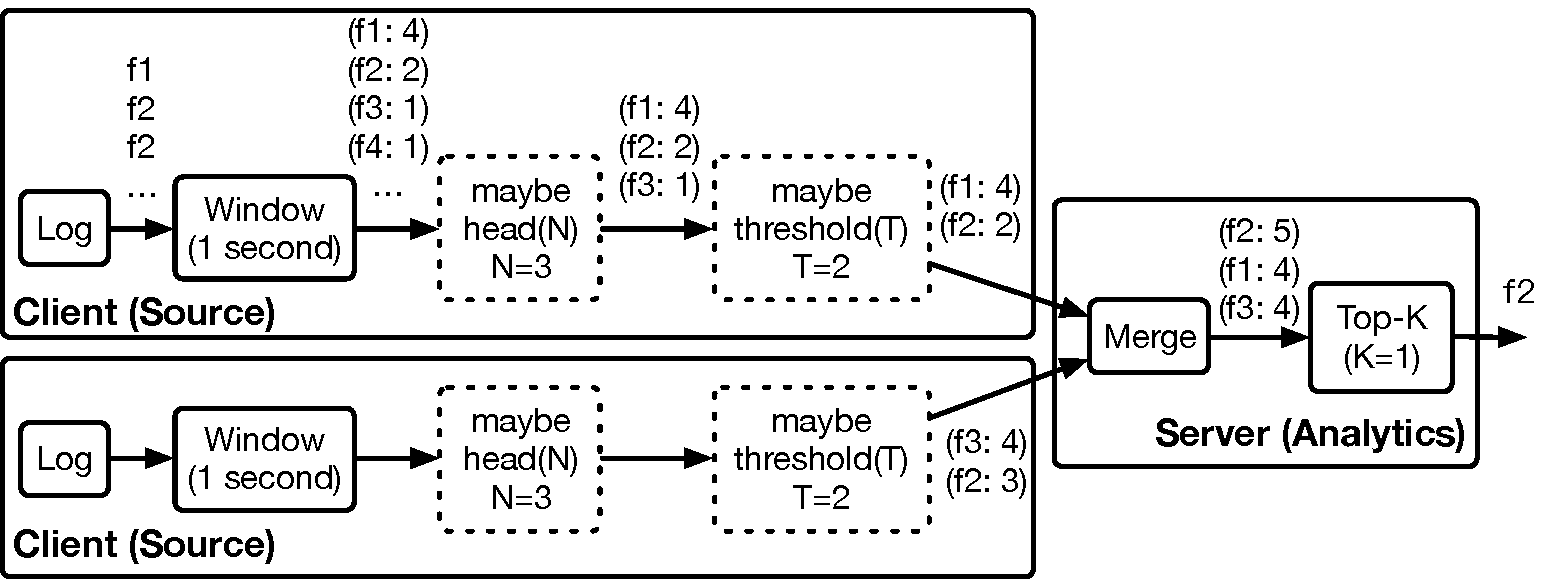
\includegraphics[width=\columnwidth]{figures/topk.pdf}
  \caption{A distributed Top-K application with two degradation operations:
    \texttt{head} and \texttt{threshold}.}
  \label{fig:topk}
\end{figure}

Naively aggregating all the raw logs is not feasible because popular servers
have millions of requests per second. Edge nodes can first perform a
\texttt{Window} operation to generate data summary, such as key-value pairs of
\texttt{<item, count>}. Even after this operation, however, the data size can
still be too large because most real-world access patterns follow a long tail
distribution. There is a large-but-irrelevant tail that contributes little to
the final results.

The edge nodes perform two degradation operations: (1) a head (\texttt{N})
operation that only takes the top \texttt{N} entries; (2) a threshold \texttt{T}
that filters small entries. These two operations are not orthogonal. Their
impact on data size reduction and quality degradation depends on the data
distribution. For the accuracy function, we use
Kendall's~$\tau$~\cite{abdi2007kendall}, a correlation measure of the
concordance between two ranked list. The output ranges from \(-1\) to 1,
representing no agreement to complete agreement. To integrate with \sysname{},
we convert Kendall's~$\tau$ to the range of [0, 1] with a linear transformation.

Our Top-K application aims to find the fifty most accessed files from web server
logs. We use Apache log files that record and store user access statistics for
the \href{https://www.sec.gov}{SEC.gov} website. We split these logs into four
groups, simulating four geo-distributed nodes monitoring web accesses.  To match
the load of popular web servers, we compress one hour's logs into one second.

\section{Runtime Experiments}
\label{appendix:more-runtime}

\todo{Report Ping times.}

In this section, we show the runtime experiments for other two applications:
pedestrians detection and Top-K analysis.

\begin{figure}
  \centering
  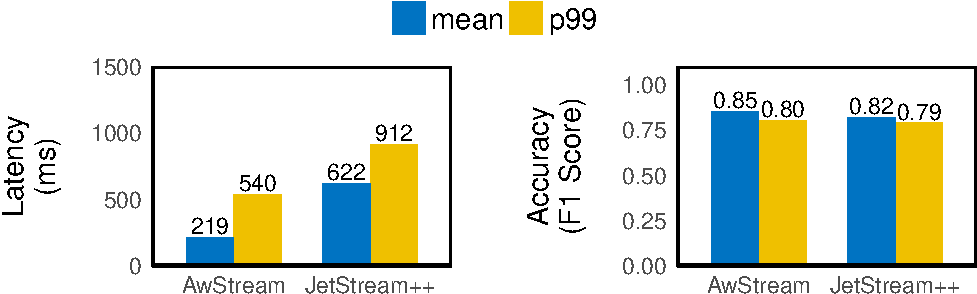
\includegraphics[width=0.95\columnwidth]{figures/mot-runtime-bar.pdf}
  \caption{Pedestrian Detection. \sysname{} in comparison with JetStream++.}
  \label{fig:mot-runtime-bar}
\end{figure}

\begin{figure*}[htb]
  \centering
  \begin{subfigure}[t]{0.45\textwidth}
    \centering
    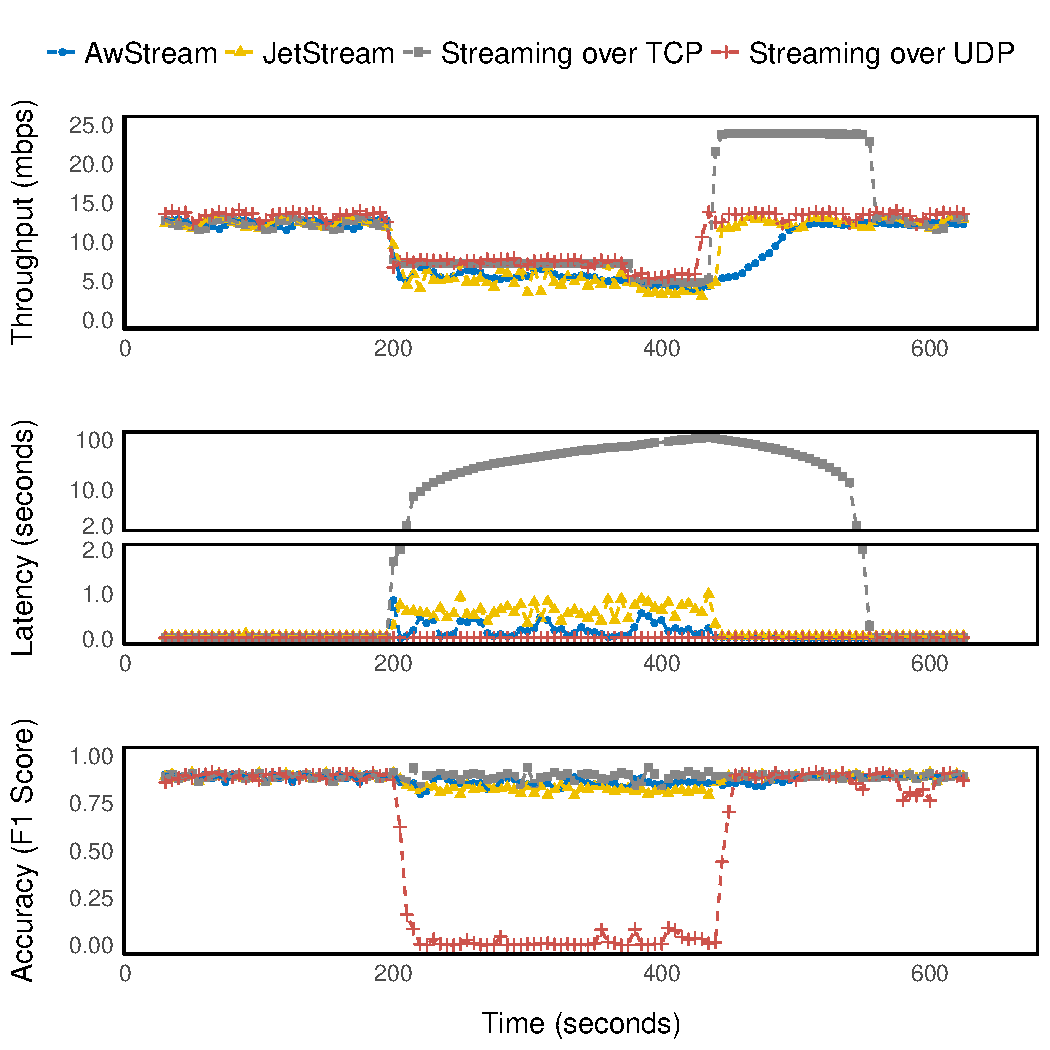
\includegraphics[width=\columnwidth]{figures/runtime-mot-verticle.pdf}
    \caption{Runtime behavior of PD application.}
    \label{fig:pd-runtime}
  \end{subfigure}
  \hfill
  \begin{subfigure}[t]{0.45\textwidth}
    \centering
    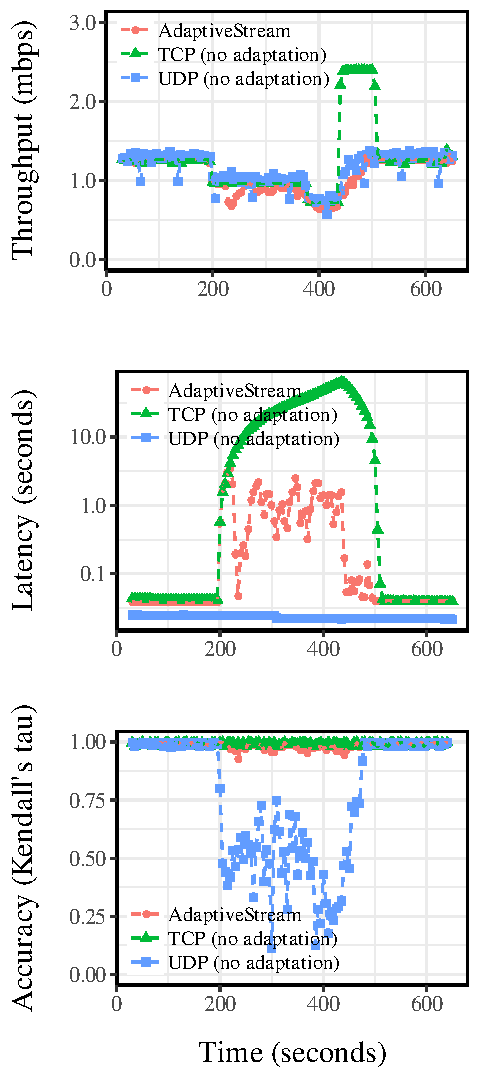
\includegraphics[width=\columnwidth]{figures/runtime-topk-verticle.pdf}
    \caption{Runtime behavior of TK application.}
    \label{fig:tk-runtime}
  \end{subfigure}
  \caption{Application profiles of three applications. Each cross point is one
    configuration $c$'s performance $(B(c), A(c))$. All figures show the Pareto
    boundary as well as the performance if only tuning one dimension. Note the
    x-axis is in log scale.}
  \label{fig:all-profiles}
\end{figure*}

\begin{figure}
  \centering
  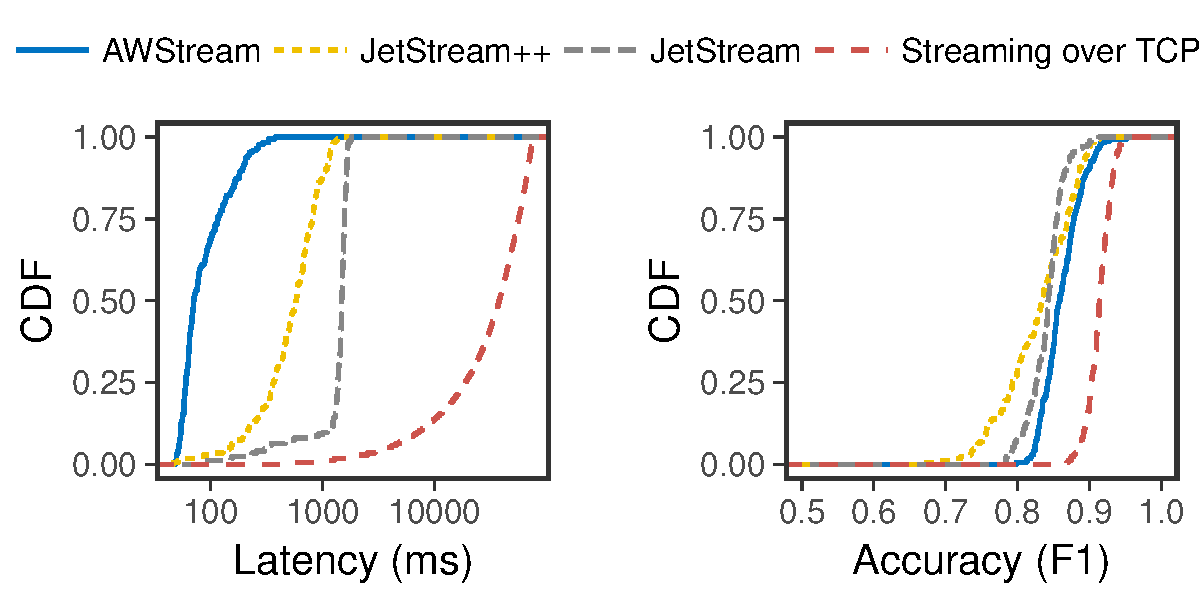
\includegraphics[width=0.95\columnwidth]{figures/runtime_mot-cdf.pdf}
  \caption{\sysname{}}
  \label{fig:darknet-runtime-cdf}
\end{figure}

\section{JetStream++}
\label{appendix:jetstream++}

We modified the open source version of
JetStream\footnote{\url{https://github.com/princeton-sns/jetstream/}, commit
  bf0931b2d74d20fdf891669188feb84c96AF84} in order to use our profile to act as
manual policies. Because JetStream doesn't support simultaneous degradation in
multiple dimensions, we implemented a simple \texttt{VideoSource} operator that
understands how to change image resolutions, frame rate, and video encoding
quantization. At runtime, \texttt{VideoSource} queries congestion policy manager
and adjusts three dimensions simultaneously. This operator is then exposed to
Python-implemented control plane. The JetStream implementation is quite modular
and extensible: the modifications include 53 lines for the header file, 171
lines for implementation, 75 lines for unit test, and 49 lines of python as the
application. But the resulting implementation loses the composability of what
\sysname{} provides for different operators.

We did not implement the Top-K application because we believe the video
analytics is enough to illustrate the difference between JetStream and
\sysname{}. Although JetStream does provide a Top-K implementation, it is based
on ``Three-Phase Uniform Threshold'' (TPUT) and not suitable for low-latency
Top-K monitoring, according to the original paper~\cite{cao2004efficient},
\textit{``in our target environments the query is asked hourly or daily. The
  intervals between the queries are typically long enough that the top-k objects
  have changed completely.''}

%% https://github.com/nebgnahz/jetstream-clone/pull/2/files

%%% Local Variables:
%%% mode: latex
%%% TeX-master: "awstream"
%%% End:
